\section{Esamų sistemų pertvarkymas}
Apsibrėžus šablonus paketų skirstymui galima pradėti vertinti jų efektyvumą, juos pritaikant esamoms sistemoms.
Šio skyriaus tikslas pasirinkti ir išnagrinėtis kelias sistemas, pasitelkus paketų kokybes metrikas, bei bendra sistemos struktūros analizė,
taip identifikuojant programiniam kodui būdingas problemas, rastas problemas išspręsti pritaikant aprašytūs šablonus.
Atlikus pertvarkymus sistemose, dar kartą paskaičiuoti paketų kokybės metrikas, taip gaunant įrodymus ar gauti šablonai yra efektyvus ir ištikrūjų sprendžia
jiems priskirtas problemas.


\subsection{Sistemų pasirinkimas}
Sistemų pertvarkymui pasiritinktos trys atviro kodo sistemos, kurių kodas yra viešai prietinamas \textit{github} platformoje.
Pasirinktos sistemos yra vidutinio dydžio, todėl nėra labai sudėtinga jas suprasti ir pertvarkyti, bet taip pat jos nėra
tokios paprastos, kad neturėtų sistemos dizaino problemų.
Pasirenktos sistemos yra skirtingo tipo projektai, taip užtikrinant
didesnę problemų ivairovę.
Pasirinktos sistemos:
\begin{itemize}
    \item \textbr{Leaf\footnote{\url{https://github.com/Meituan-Dianping/Leaf/tree/master}}} - sistema per \textit{http}
    protokolą teikiantį aplikacijų programavimo sąsają,
    unikalaus identifikatoriaus generavimui, taip užtikrinant jo unikalų pasiskirstymą, tarp skirtingų paskirstytos sistemų \angl{distributed systems},
    servisais orientuotoje \angl{service-oriented} architektūroje.
    Tai techninės programinės įrangos tipas, kuris naudojamas kitų taikomosios programinės įrangos sistemų.
    \item
\end{itemize}
• Taikomoji programinė įranga, teikianti paslaugas įrangos naudotojams. Pavyzdžiui,
internetinė programėlė priminimams ir darbams užsirašyti
• Programinės įrangos įrankiai, skirti naudoti kitose sistemose supaprastinant programinį
kodą, naudojant jau įgyvendintas funkcijas. Pavyzdžiui, Java programavimo kalbos
Spring karkasas internetinių programėlių kūrimui


\subsection{\textit{Leaf} sistemos pertvarkymas}
Sistema Leaf susidėda iš dvieju modulių \textit{server} ir \textit{core}, šiame darbe dėmesys bus skirtas tik \textit{core} moduliui, kadangi \textit{server} modulis yra labai mažas
ir paketų struktūra jame neatlieka esminio vaidmens.
Prieš visus pakeitimus \textit{Leaf} sistemos, \textit{core} modulio paketų struktūra atrodo taip:
\begin{figure}[H]
    \centering
    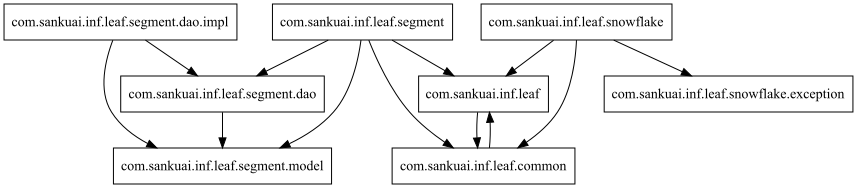
\includegraphics[scale=0.15]{img/leaf_packages_orig}
    \caption{\textit{Leaf} sistemos \textit{core} modulio struktūra}
    \label{img:leaf_packages_orig}
\end{figure}

\dirtree{%
.1 {/} .
.2 {com}.
.3 {sankuai}.
.4 {inf}.
.5 {leaf}.
.6 {common}.
.6 {segment}.
.7 {dao}.
.8 {impl}.
.7 {model}.
.6 {snowflake}.
.7 {exception}.


\begin{center}
    \begin{tabular}{|c|c|c|c|c|c|c|}
        \hline
        Paketo vardas & \textit{N} & \textit{A} & \textit{E} & \textit{S} & \textit{A} & \textit{D} \\ [0.5ex]
        \hline\hline
        com.sankuai.inf.leaf.segment.dao.impl & 1 & 0 & 8 & 1.0 & 0.0 & 0.0 \\
        \hline
        com.sankuai.inf.leaf.segment & 1 & 0 & 10 & 1.0 & 0.0 & 0.0 \\
        \hline
        com.sankuai.inf.leaf.snowflake.exception & 3 & 1 & 0 & 0.0 & 0.0 & 1.0 \\
        \hline
        com.sankuai.inf.leaf.segment.model & 3 & 3 & 3 & 0.5 & 0.0 & 0.5 \\
        \hline
        com.sankuai.inf.leaf.segment.dao & 2 & 2 & 3 & 0.6 & 1.0 & 0.6 \\
        \hline
        com.sankuai.inf.leaf & 1 & 3 & 1 & 0.25 & 1.0 & 0.25 \\
        \hline
        com.sankuai.inf.leaf.common & 6 & 3 & 5 & 0.625 & 0.0 & 0.375 \\
        \hline
        com.sankuai.inf.leaf.snowflake & 2 & 0 & 17 & 1.0 & 0.0 & 0.0 \\
        \hline
    \end{tabular}
    \begin{tabular}{|c|c|c|c|c|c|}
        \hline
        $\bar{N}$ & $\bar{A}$ & $\bar{E}$ & $\bar{S}$ & $\bar{A}$ & $\bar{D}$ \\ [0.5ex]
        \hline\hline
        2 & 2 & 6 & 0.622 & 0.25 & 0.341 \\
        \hline
    \end{tabular}
\end{center}
